De logs zijn stukjes tekst die een systeem genereert op basis van gebeurtenissen. Als er bijvoorbeeld een gebruiker inlogt kan het systeem een bericht (log) genereren dat de gebruiker succesvol is ingelogd.

Een systeem maakt verschillende soorten log berichten aan. De berichten kunnen gaan over het systeem, over de beveiliging of over applicaties. Als er een probleem is met het besturingssysteem of een applicatie is Event Viewer vaak de eerste plek om te gaan zoeken.

De logs bevatten informatie over wat er gebeurd is en de datum en het tijdstip waarop de gebeurtenis heeft plaatsgevonden. Ook kunnen ze foutcodes bevatten waarop je op Internet kunt zoeken naar meer informatie en mogelijke oplossingen.

Om deze logs te kunnen bekijken is er een MMC-module met de naam Event Viewer\index{event viewer}\index{mmc!event viewer} (Logboeken\index{logboeken}\index{mmc!logboeken}. Met Event Viewer kan je ook logs beheren.

Binnen Event Viewer ...
is ingedeeld in categorieën zoals Windows-logboeken, toepassings- en serviceslogboeken en abonnementen. Gebruikers kunnen logboeken filteren op criteria zoals gebeurtenisniveau, datum en trefwoorden om snel relevante gebeurtenissen te vinden. Met de Logboeken kunnen gebruikers ook logboekbestanden opslaan voor analyse en gebeurtenisgegevens exporteren voor extern gebruik.

Voor IT-professionals is de Logboeken een krachtig hulpprogramma voor het diagnosticeren van problemen, het controleren van systeemactiviteiten en het garanderen van naleving van beveiligingsbeleid. Het wordt ook gebruikt om de status en status van servers en andere kritieke infrastructuuronderdelen bij te houden.

Om Event Viewer te openen zijn er verschillende manieren:
\begin{itemize}
\item
	\begin{enumerate}
		\item Start MMC
		\item Selecteer in het File menu Add/Remove snap-in
		\item Selecteer Event Viewer en klik op Add
	\end{enumerate}
\item Gebruik de windows-toets + r en run eventvwr.msc\index{eventvwr.msc}
\item Klik op het zoek icoon en zoek op Event Viewer
\end{itemize}

%% \begin{minipage}[t]{\linewidth}
%% \raggedright
%% \adjustbox{valign=t}{%
%% 	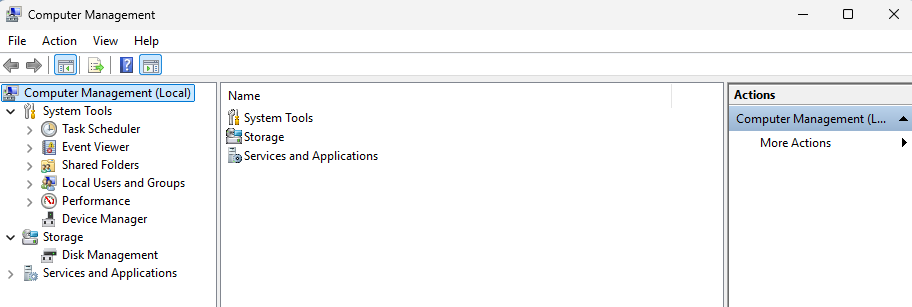
\includegraphics[width=0.99\linewidth]{computermanagement.png}%
%% }
%% \end{minipage}

